\documentclass[]{book}
\usepackage{amsmath,amssymb}
\usepackage{amsthm}
\usepackage{xpatch}
\xpatchcmd\swappedhead{~}{.~}{}{}

\usepackage[T1]{fontenc}
\usepackage[utf8]{inputenc}

\usepackage{parskip}
\usepackage{lmodern}
\usepackage{verbatim}
\usepackage{enumerate}
\usepackage{longtable}
\usepackage{booktabs}


\usepackage{xcolor}
%sudo apt-get install texlive-pictures
\usepackage[all]{xy}

\usepackage{hyperref}

\usepackage[ marginparwidth=3cm, marginparsep=0cm]{geometry}
\usepackage{graphicx}
\usepackage[spanish]{babel}


% Scale images if necessary, so that they will not overflow the page
% margins by default, and it is still possible to overwrite the defaults
% using explicit options in \includegraphics[width, height, ...]{}
\setkeys{Gin}{width=\maxwidth,height=\maxheight,keepaspectratio}
% Set default figure placement to htbp
\makeatletter
\def\fps@figure{htbp}
\makeatother


\providecommand{\tightlist}{%
  \setlength{\itemsep}{0pt}\setlength{\parskip}{0pt}}

  
%remove section numbers
%\setcounter{secnumdepth}{0}

\title{Variables aleatorias continuas}
\author{Hugo J. Bello}
\date{}


\renewcommand{\familydefault}{\sfdefault}
\setcounter{chapter}{4}


\theoremstyle{plain}
\swapnumbers % Switch number/label style
\newtheorem{theorem}{Theorem}[section]
\newtheorem{corollary}[theorem]{Corollary}
\newtheorem{lemma}[theorem]{Lemma}
\newtheorem{claim}{Claim}[theorem]
\newtheorem{axiom}[theorem]{Axiom}
\newtheorem{conjecture}[theorem]{Conjecture}
\newtheorem{fact}[theorem]{Fact}
\newtheorem{hypothesis}[theorem]{Hypothesis}
\newtheorem{assumption}[theorem]{Assumption}
\newtheorem{proposition}[theorem]{Proposition}
\newtheorem{property}[theorem]{Propiedad}
\newtheorem{properties}[theorem]{Propiedades}
\newtheorem{criterion}[theorem]{Criterion}
\theoremstyle{definition}
\newtheorem{definition}[theorem]{Definición}
\newtheorem{note}[theorem]{Nota}
\newtheorem{definitions}[theorem]{Definiciones}
\newtheorem{example}[theorem]{Ejemplo}
\newtheorem{remark}[theorem]{Remark}
\newtheorem{problem}[theorem]{Problem}
\newtheorem{principle}[theorem]{Principle}
\newtheorem{method}[theorem]{Método}
\newtheorem{exercise}[theorem]{Ejercicio}

% for specifying a name
\theoremstyle{definition} % just in case the style had changed
\newcommand{\thistheoremname}{}
\newtheorem{genericthm}[theorem]{\thistheoremname}
\newenvironment{customdef}[1]
  {\renewcommand{\thistheoremname}{#1}%
   \begin{genericthm}}
  {\end{genericthm}}


\begin{document}




\maketitle

\section{Variables aleatorias continuas, definición y
propiedades} 

Recordemos que habíamos definido \textbf{variable aleatoria} es
esencialmente un número aleatorio.

Hasta ahora hemos trabajado con variables aleatorias \(X\) que toman un
conjunto discreto de valores, como por ejemplo resultado de tirar un
dado. Sin embargo en muchas ocasiones nuestras variables tomarán un
conjunto continuo de valores, como puede ser \emph{la altura de una
persona} o su peso.

Para ello introducimos las variables aleatorias continuas.


\begin{definition}
  Decimos que una variable aleatoria \(X\) es \textbf{continua} si existe
una función \(f:\mathbb R \to \mathbb R\) tal que para todos \(a\leq b\)
números reales

\[\displaystyle P(a\leq X\leq b)=\int _{a}^{b}f(x)\,dx\]

La función \(f\) se le denomina \textbf{función de masa de probabilidad}
y debe cumplir:

\begin{itemize}
\tightlist
\item
  \(f(x)\geq 0\) para todo \(x\)
\item
  \(\int^\infty_\infty f(x)dx\) = 1
\end{itemize}

Recordemos la integral es el area bajo la curva de \(f\)

\end{definition}


\begin{figure}
  \centering
  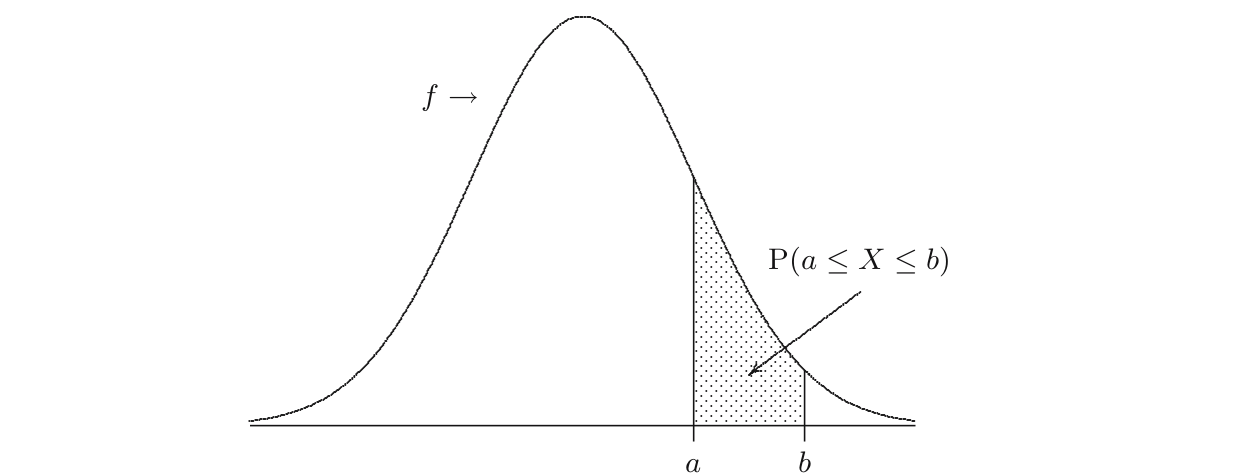
\includegraphics[width=5in,height=\textheight]{img/sc_1.png}
  \caption{ }
\end{figure} 


\begin{definition}
  Definimos al \textbf{función de distribución acumulada}, del mismo modo que
hicimos con variables discretas, pero usando ahora la integral:

\[F(x)=P(X\leq x)=\int _{-\infty }^{x}f(t)\,dt\]

\end{definition}

\subsection{Esperanza y varianza de variables continuas} 

\begin{definition}
  Para una variable aleatoria continua X con función de densidad
\(\displaystyle f(x)\) \textbf{el valor esperado o esperanza matemática}
se define como la integral

\[\displaystyle \operatorname {E} [X]=\int^{\infty}_{-\infty }xf(x)dx\]

Si recordamos es la misma idea que con variable discreta, pero en vez de
sumar integramos
\end{definition}

Al igual que ocurría con variables aleatorias discretas, en el caso continuo se cumple 

\begin{property}
  Si $X$ es una variable aleatoria continua con esperanza finita entonces se cumple que 
  \[E[a + b \cdot X] = a + b \cdot E(X)\] para cualesquiera números reales $a,b$.
\end{property}


\begin{definition}
  La \textbf{varianza} es una medida de dispersión de una variable aleatoria X respecto a su esperanza $E[X]$ y se define como la esperanza de la transformación $(X - E[X])^2$ es decir:
  
  \[Var[X]= E[(X- E[X])^2] = \int^{\infty}_{-\infty }(x-E[X])^2f(x)dx\]
\end{definition}


\begin{property}
  Si $X$ es una variable aleatoria continua con esperanza finita entonces se cumple que 
   \[
    \operatorname {Var} (X) =\operatorname {E} \left[X^{2}\right]-\operatorname {E} [X]^{2} 
 \]
\end{property}

\subsection{La distribución
uniforme} 

Una variable aleatoria continua tiene una distribución uniforme en el
intervalo \([\alpha, \beta]\) si función de densidad es la siguiente

\[f(x)=\begin{cases}{\frac {1}{\beta-\alpha}}&\mathrm {para} \ \alpha\leq x\leq \beta,\\[8pt]0&\text {para el resto de valores}\end{cases}\]

Se denota por \(U(\alpha, \beta)\).

Si calculamos la distribución acumulada:

\[F(x)= \int _{-\infty }^{x}f(t)\,dt\]

veremos que el resultado es

\[\displaystyle F(x)=\begin{cases}0&{\text{para }}x<a\\[8pt]{\frac {x-a}{b-a}}&{\text{para }}a\leq x\leq b\\[8pt]1&{\text{para }}x>b\end{cases}\]
 

\begin{figure}[htbp]
  \begin{minipage}{0.5\linewidth}
  \centering
  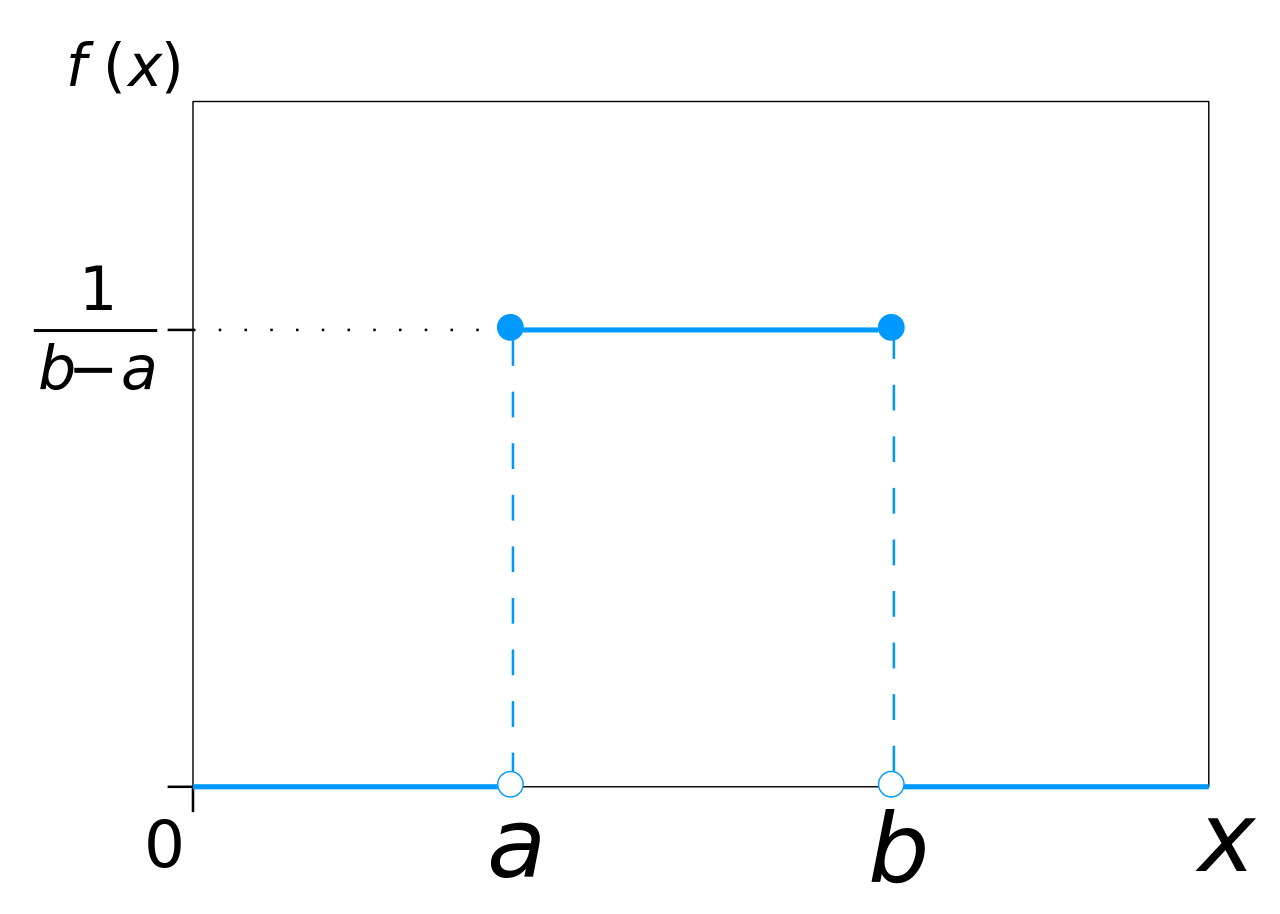
\includegraphics[width=2in,height=\textheight]{img/uniform.png}
  \caption{Función de densidad de la distribución\\ unifome}
  \end{minipage}%
  \begin{minipage}{0.5\linewidth}
  \centering
  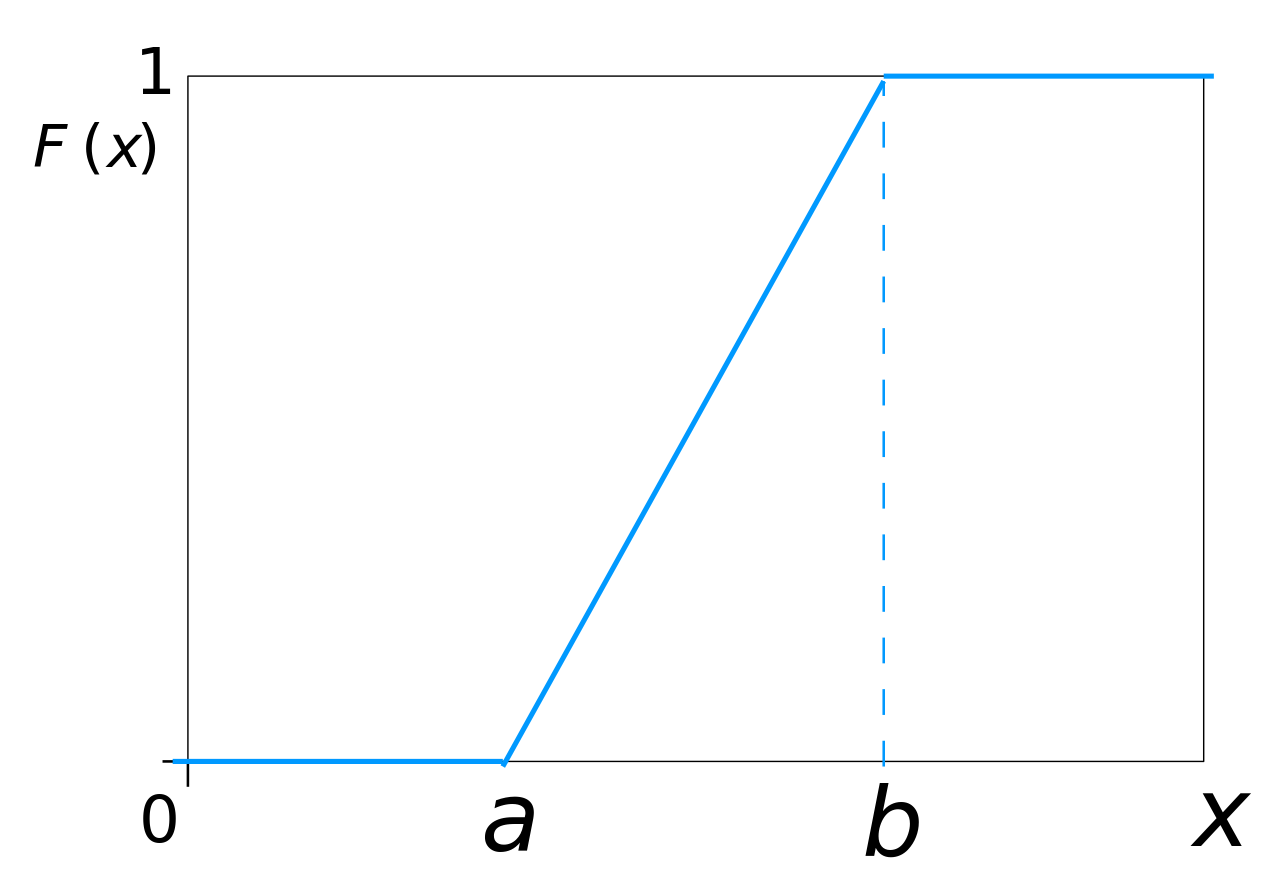
\includegraphics[width=2in,height=\textheight]{img/uniform2.png}
  \caption{Función de densidad acumulada de \\la distribución unifome}
  \end{minipage}

\end{figure} 

\begin{example}
  Para una variable  $\displaystyle X\sim U(0,23)$


  Calculemos $\displaystyle  P(2<X<18)$:

   \[\displaystyle P(2<X<18)=\int^{18}_2 \frac {1}{23-0} dx 
   =  \frac {x}{23-0} \bigg]^{18}_2 =  (18-2)\cdot {\frac {1}{23}}={\frac {16}{23}} \]
\end{example}

\begin{example}
La ruleta de la suerte tiene 20 premios repartidos en sectores iguales entre los 360 grados del círculo. Al empujar el 
la ruleta gira y finaliza al azar en cualquiera de los ángulos de giro. 
Que acabe en un ángulo concreto sigue una distribución uniforme U(0, 360). 
Calcular la probabilidad de que caiga el premio situado entre los ángulos 0 y 18 grados.
 

\[\displaystyle P(0<X<18)=\int^{18}_0 \frac {1}{360-0} dx 
=  \frac {x}{360} \bigg]^{18}_0 =  (18-0)\cdot {\frac {1}{360}}={\frac {18}{360}} \]

\end{example}

\begin{property}
  Si $X \sim  U(\alpha, \beta)$ entonces 
  \begin{enumerate}
    \item $E[X] = \frac{1}{2} (\alpha+\beta)$
    \item $V[X] = \frac{1}{12} (\beta-\alpha)$
  \end{enumerate}
\end{property}

\begin{proof}
  Para ver (1), basta calcular 
  \[E[X] = \int^{\beta}_{\alpha} x \frac{1}{\beta - \alpha} dx 
  = \bigg[\frac{x^2}{2}\bigg]^{\beta}_{\alpha}\frac{1}{\beta - \alpha}  =  \frac{\beta^2-\alpha^2}{2(\beta - \alpha)}
  = \frac{(\beta-\alpha)(\beta + \alpha)}{2(\beta - \alpha)} = \frac{1}{2} (\alpha+\beta) \]
  Para demostrar (2) usaremos que $E[X^2] = \frac{\beta^3 - \alpha^3}{3\beta - 3\alpha}$, esto se puede demostrar usando una integral similar a la anterior. 
  Ahora vemos que 
  \begin{align*}
    V[X] &= E[X^2] - E[X]^2 = \frac{\beta^3 - \alpha^3}{3\beta-3\alpha} - \frac{(\alpha+\beta)^2}{4} \\
    &= \frac{4(\beta^3 - \alpha^3) - 3(\beta-\alpha)(\alpha+\beta)^2}{12(\beta-\alpha)} \\
    &= \frac{(\beta-\alpha)^3}{12(\beta - \alpha)} = \frac{1}{12} (\beta-\alpha)
  \end{align*}
 
\end{proof}

\subsection{La distribución normal} 

La distribución normal juega un rol central en la teoría de la
probabilidad y la estadística. Una de sus aplicaciones se debe a C.F.
Gauss, que la usó en 1809 para medir errores en astronomía.

Una función aleatoria continua tiene una \textbf{distribución normal}
con parámetros \(\mu\) y \(\sigma\), su función de densidad de
probabilidad es

\[f(x) = \frac{1}{\sigma \sqrt{2\pi}} e^{-\frac{(x-\mu)^2}{2\sigma^2}}\]

Esta distribución se denota por \(N(\mu, \sigma)\).


\begin{figure}
  \centering
  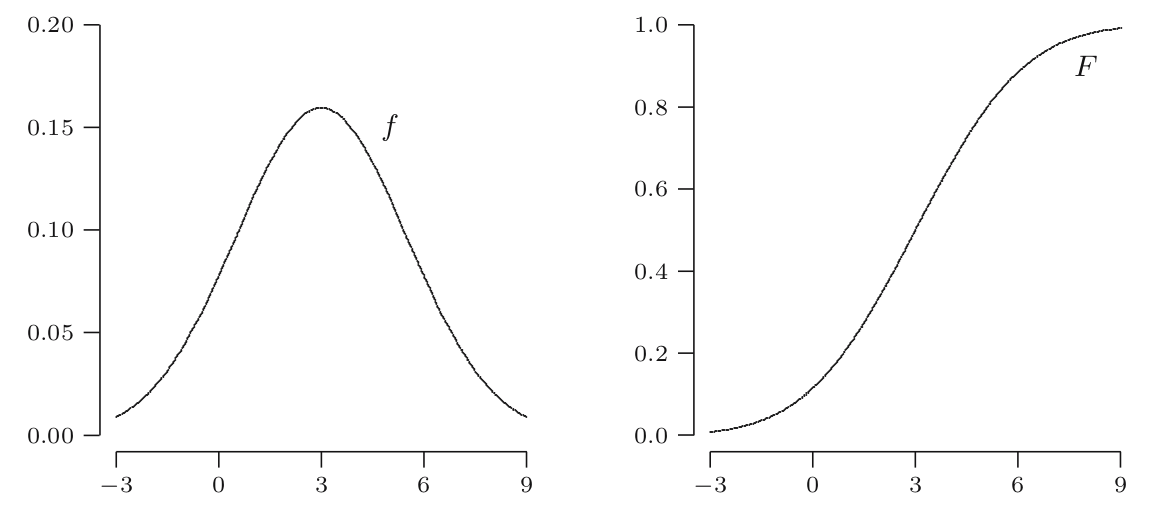
\includegraphics[width=4in,height=\textheight]{img/sc_3.png}
  \caption{ }
\end{figure}


Como vemos esta función \(f\) tiene una forma de campana, donde los
parámetros \(\mu\) y \(\sigma\) se interpretan como:

\begin{itemize}
\item
  \(\mu\) determina el valor entorno al que se centra la campana.
  Veremos que coincide con la esperanza matemáticas.
\item
  \(\sigma\) determina lo \emph{apretada} que está la campana, es decir
  lo dispersa que está la variable.
\end{itemize}

En la siguiente gráfica vemos la normal para distintos valores de
\(\mu\) y \(\sigma\)


\begin{figure}
  \centering
  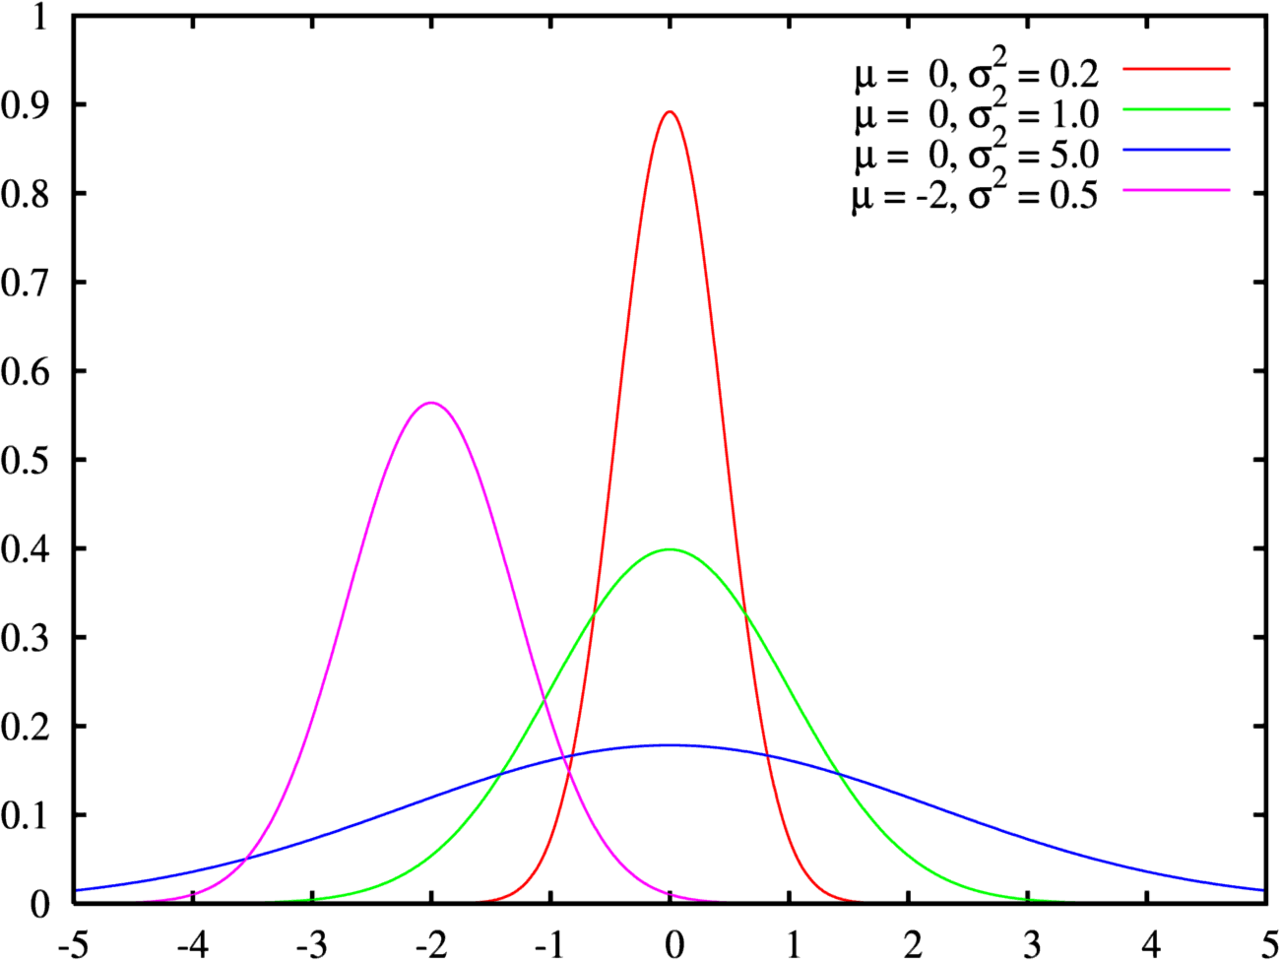
\includegraphics[width=3in,height=\textheight]{img/normal2.png}
  \caption{ }
\end{figure}
 

Algunos ejemplos de variables asociadas a fenómenos naturales que siguen
el modelo de la normal son:

\begin{itemize}
\item
  caracteres morfológicos de individuos como la estatura;
\item
  caracteres fisiológicos como el efecto de un fármaco;
\item
  caracteres sociológicos como el consumo de cierto producto por un
  mismo grupo de individuos;
\item
  caracteres psicológicos como el cociente intelectual;
\item
  nivel de ruido en telecomunicaciones;
\item
  errores cometidos al medir ciertas magnitudes;
\end{itemize}

\hypertarget{bibliografuxeda}{%
\section{Bibliografía}\label{bibliografuxeda}}

\begin{itemize}
\tightlist
\item
  John A. Rice. Mathematical Statistics and Data Analysis
\item
  F. M. Dekking, C. Kraailkamp, H. P. Lopuhaa, L. E. Meester. A Modern
  Introduction to Probability and Statistics. Understanding Why and How.
\end{itemize}

\end{document}